\chapter{Introduction}

\section{Abstract}
Reverse mode differentiation builds the base for every machine learning algorithm. However, reverse mode differentiation is not trivial and therefore many ways to implement it have been and are still developed. Every implementation tries to be the best in some metric like for example easiness, speed or purity. Our main goal of this work is to show the differences and arguably more importantly the similarities between multiple implementations in written code, client API and runtime performance. For this we design our own implementations from scratch but also implement ideas developed by others and try to expand them. The comparison of code and API is done by incrementally developing each implementation by altering or referencing previous implementations to demonstrate differences/similarities on the way.

\section{Motivation}
Machine learning (ML) is a big research area in computer science. Much research on ML is done either directly or indirectly by using it to achieve some other goal/knowledge (e.g. for image recognition or natural language processing). Research on computer languages concerning problems specific to ML could facilitate the implementation of ML applications for many use cases.  Gradient descent and therefore differentiable programming builds the base of ML which makes it the perfect target for research because better implementations could lead to improvements in many applications of ML. Having an overview of possible implementations would make it possible to decide which implementation is best suited to design a ML library, algorithm or even (domain specific) language.

Our goal for this work is to produce such an overview by implementing differentiation in multiple ways. These will be partly based on other's work which we (re-)implement and adjust to fit a similar implementation style so that we can easily compare all implementations. Furthermore, we will extend those implementations with new functionalities, change them from the ground up or implement our own designs from scratch. Secondarily we will try to find use cases of the new language features introduced in Scala 3 to get an idea if this language has potential to aid implementing ML tasks.

\section{Overview}
We provide 10 distinct implementations of differentiation which are based on various (sometimes combined) concepts. 3 of those implement forward mode differentiation where we use simple operator overloading but also experiment with more advanced features like macros. Reverse mode differentiation has 4 implementations which use mutation and 3 which follow a more pure approach. Ubiquitous concepts used for this are tapes to store operations, continuation passing style programming and monads.

In detail, we start off with implementing the normal well-known forward mode differentiation in \refsec{sec:forwardMode}. For this we first give a quick view on how to use a naive but unorthodox way to implement it using macros to replace code in \refsec{sec:macros}. After that we introduce the more common dual numbers in \refsec{sec:forwardDualNumbers} which will be a key ingredient also for later (reverse mode) implementations. The next implementation gets more experimental again. In \refsec{sec:matchTypes} we use the newly introduced match types and value types of Scala 3 to implement a symbolic differentiation-like way to produce a derivative completely at type level in compile time.

The main focus of this work is reverse mode differentiation (\refsec{sec:reverseMode}) which is much more relevant for ML tasks than forward mode. Here we begin by introducing the mathematical background of reverse mode by doing it once ``by hand''. This section is divided into two main parts. One where we use mutation (\refsec{sec:mutation}) and one where we refrain from using it (\refsec{sec:noMutation}).

As using mutation and non-functional programming usually leads to an arguably more straight forward implementation we for now continue without restricting us to functional programming in \refsec{sec:mutation}. We introduce continuation passing style (CPS) which at first seems like unnecessary overhead and in itself may be hard to wrap your head around at first. However, it pays off when it elegantly demystifies how to implement reverse mode differentiation in \refsec{sec:cps}. Using a tape to store operations on in \refsec{sec:tape} is also a valid way to implement reverse mode in a similar way to CPS. From there we continue by wrapping CPS into a monad in \refsec{sec:monadCPS} to facilitate usage of CPS from the client side. We finish the mutation section by combining the monad and tape idea in \refsec{sec:monadAndTape}.

For the more puristic oriented in \refsec{sec:noMutation} we translate the CPS and monad implementations in \refsec{sec:functionalCps} and \refsec{sec:functionalMonad} respectively into a design which does use an accumulator which maps expressions to their adjoints instead of using mutation. The last implementation (in \refsec{sec:chad}) is fully functional and does not even need a unique ID per expression which consequently means it only needs value equality to work. On top of that it is easily comprehensible because it comes without much overhead or complicated abstractions.

In the end we will compare the runtime performance of each implementation in \refsec{sec:evaluation}.


To conclude our introduction, we want to give a quick overview over which sections are based on which external work. We based the implementations of dual numbers (\refsec{sec:forwardDualNumbers}), CPS (\refsec{sec:cps}, \refsec{sec:functionalCps}) and tape (\refsec{sec:tape}) on the work of Fei Wang et al.~\cite{lantern}. All monad based implementations (\refsec{sec:monadCPS}, \refsec{sec:monadAndTape}, \refsec{sec:functionalMonad}) are mainly based on our own work but do refer to or build on concepts introduced in the previously mentioned sections and therefore are indirectly based on the work of Fei Wang et al. They additionally use a running example function to showcase differentiation which is also used throughout our work. The work of Matthijs Vákár and Tom Smeding~\cite{chad} is the base for our CHAD implementation (\refsec{sec:chad}). The forward mode implementations using macros (\refsec{sec:macros}) and match types (\refsec{sec:matchTypes}) are implemented from scratch by us.



















% Hello
% For this work I need to cite \cite{abc12}. And \cite{tudapub}

% \section{bla}

% \subsection{blubb}

% Have a look at figure \ref{uml_example} to see how including images works.

% \begin{figure}
%     \centering
%     remember to include a path relative to your root .tex file
%     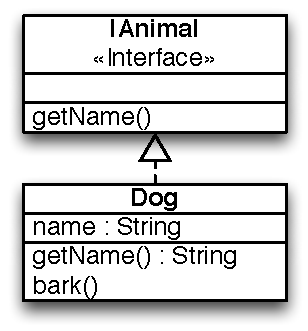
\includegraphics[width=4cm]{images/uml}
%     \caption{Sample UML Diagram}
%     \label{uml_example}
% \end{figure}

% \subsection{blubb 2}

% Avoid single subsections! Each ``parent'' has to have at least two ``childs''

% \section{bla 2}
